\item A bobina tem massa de \SI{100}{\kilogram} e raio de giração de \SI{400}{\milli\meter} em relação a seu centro de massa O. Se ela é solta do repouso, determine sua velocidade angular após seu centro $O$ haver descido pelo plano a uma distância de \SI{2}{\meter}. O coeficiente de atrito cinético entre a bobina e o plano inclinado é $\mu_{k}=\SI{.15}{}$.

\import{../answers}{answer-6}

\vspace{-1cm}
\begin{flushright}
	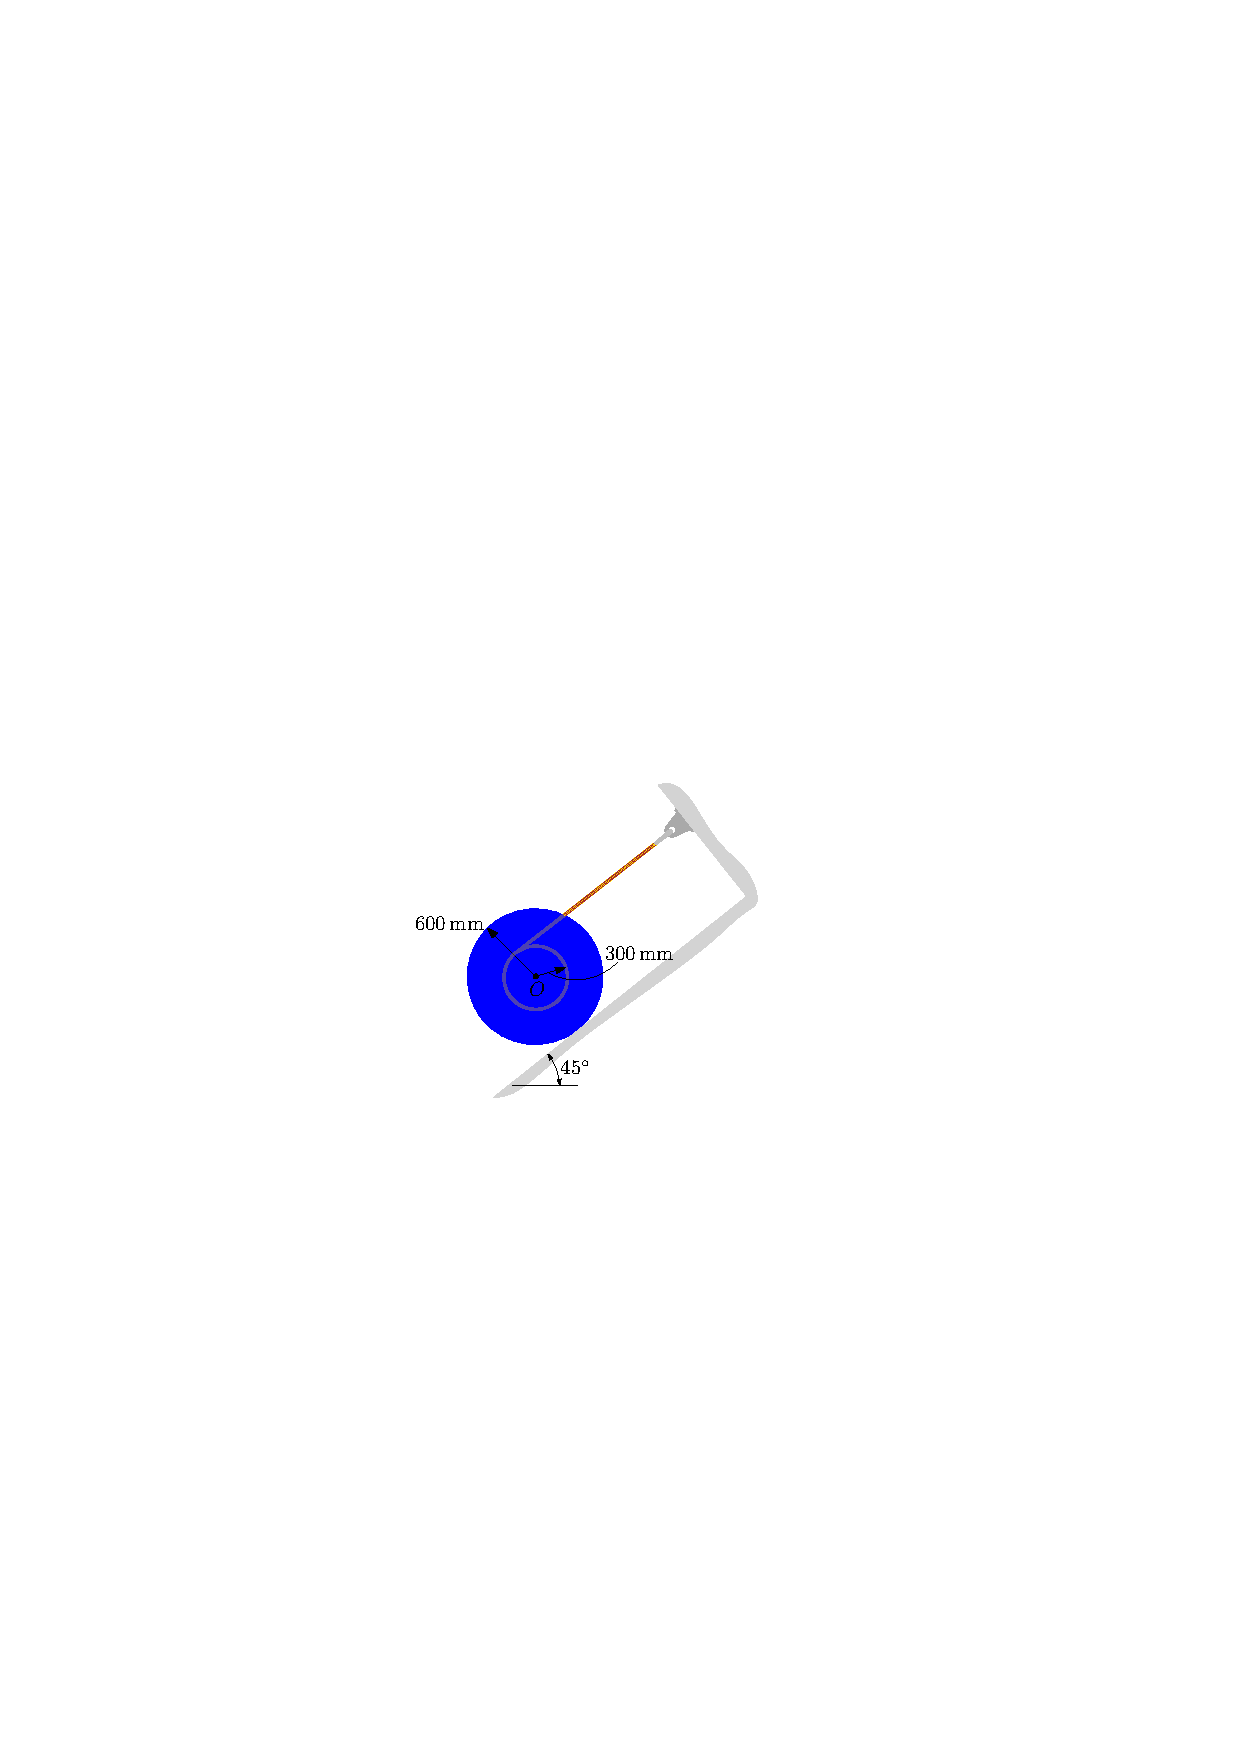
\includegraphics[scale=1.3]{../../images/draw_3_1}
\end{flushright}